\section{Box-office Predicting}
Movie box office is influenced by many factors, such as investment budget, script, director, actor, post production, producer and producer, media publicity and movie reputation. On the whole, we quantify the factors that affect movie box office from the film itself, the director, the actor and the audience. The opening week due to the lack of effective comments, so just for the release of the film at the box office during the period of life prediction problem, we consider the factors associated with the film at the box office and did not join the historic influence of sentiment analysis, in the opening week after we join in the model of the value of emotional factors.

\label{sec:predict}
\subsection{Premiere week box-office predicting}
\begin{table}[!htb]
  \centering
\begin{tabular}{|c|c|}
\hline
Symbol&Description\\
\hline
sc&\tabincell{c}{The mean bos of well-known \\ actors and directors}\\
\hline
gsc&\tabincell{c}{The mean wms of well-known \\ actors and directors}\\
\hline
std&\tabincell{c}{The variance bos of well-known \\ actors and directors}\\
\hline
gstd&\tabincell{c}{The variance wms of well-known \\ actors and directors}\\
\hline
\end{tabular}
  \caption{Features}
\end{table}
\par I film itself
\par The film's own factors include the stage of film screening, the exposure of the film media, whether it is a series of films and the type four of the film. The movie schedule is on a time, due to the holidays there will inevitably be the movie box office movie schedule or across different holidays, generally speaking, the holiday schedule has a positive impact on the movie box office; media exposure includes the program group organization during the period before the release of the film and the film series of events; is a two value variable, usually if a series of films, the box office is often influenced by the earlier film; type of film is to reflect the audience's preferences on the movie box office has a certain reference value.
\par II directors and actors factors
\par The importance of a film director to a film is self-evident. He directly determines the quality of a film, of course, the quality is not absolute. On the one hand, with the development of the commercial movie, the movie is more and more tend to cater to the preferences of the audience, however, everyone has their own views on the film art director, is no exception, this will inevitably occur between the director and the part of the audience does not agree; on the other hand, as the director of professional water products the level of production, the film quality have different gap. Therefore, we choose the word of mouth before the director as an index to measure the director's factors, and make a statistical calculation of the word-of-mouth of the historical works, so as to reflect the director's professionalism and director's strength and reputation.
\subsection{Phased Box-office Predicting}
\begin{figure}[!htbp]
\centering
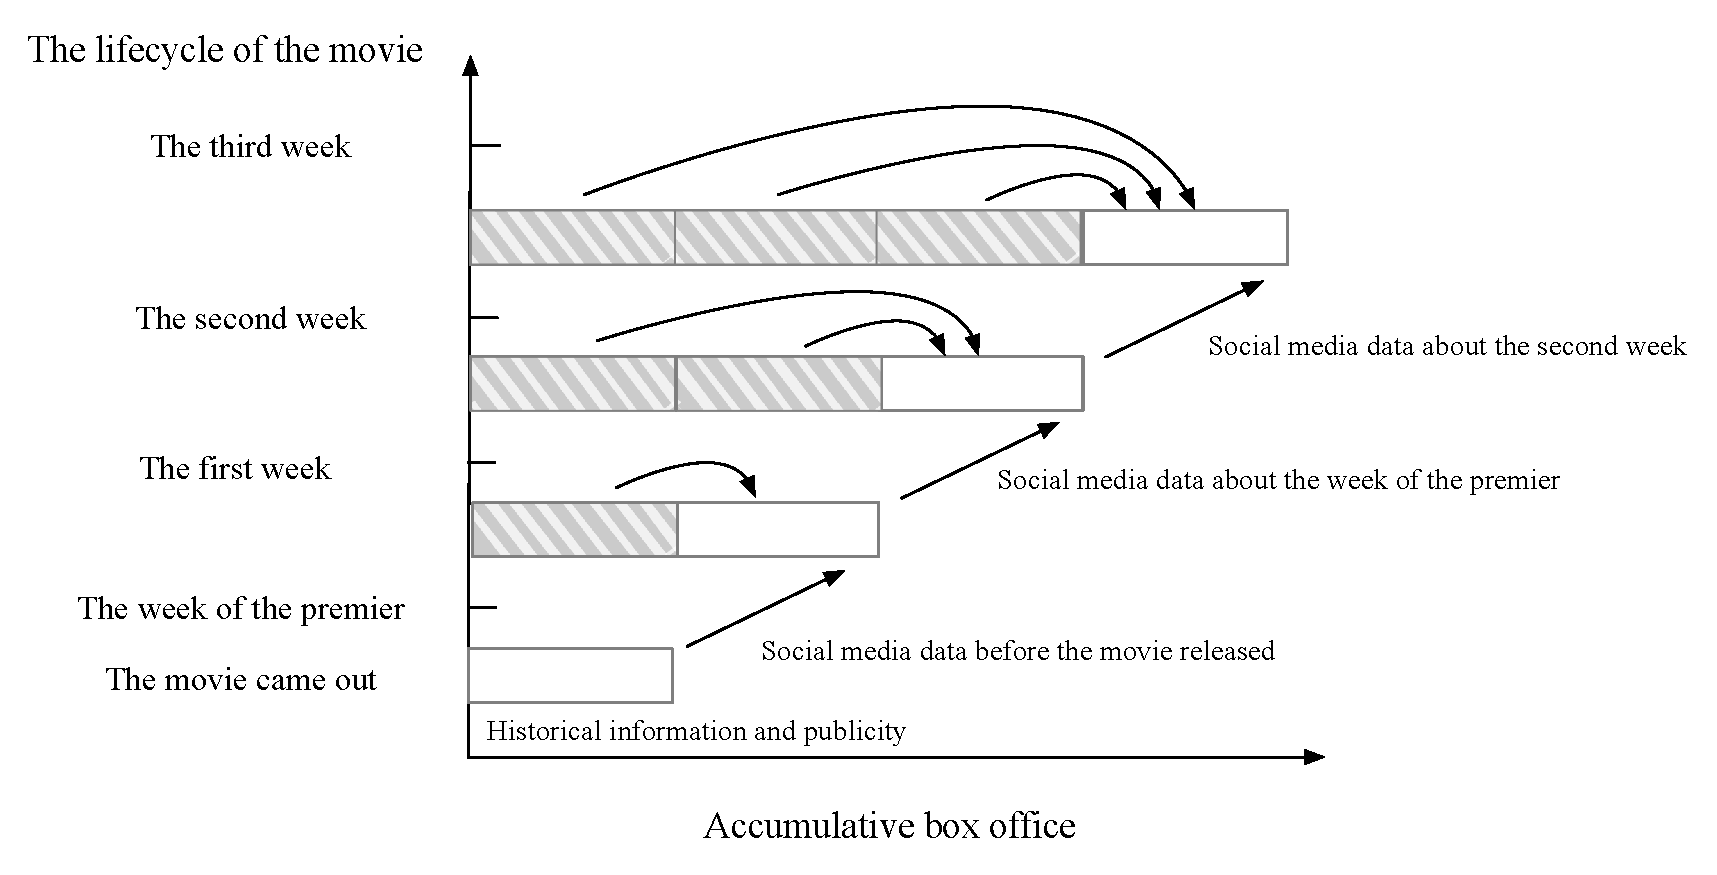
\includegraphics[width=0.8\columnwidth]{boxpredict.eps}
\caption{Multi-stage box office prediction model}
\label{fig:mhin}
\end{figure}
In the past prediction of box office, we usually only forecast the overall box office, but often ignored the movie's influence on movie box office due to the audience's attitude. Such as "wolf 2", the movie box office to be among the world's top 100, because in the release process, because the audience warmly, attracted the audience is not the original film (film series the fans, fans, like the kind of audience) to watch a movie, which leads to the box office continued to rise however, the traditional model is unable to capture this phenomenon. Therefore, from the pre launch to the 1 months after the release, we set up the box office prediction model with the weekly variation of the weekly release to predict the box office for the first week, the box office for second weeks, the third week box office and the box office at the fourth week.\\

\begin{table*}[!htbp]
\centering
\begin{tabular}{|c|c|c|c|c|c|}
\hline
\multicolumn{6}{|c|}{First Week}\\
\hline
Metric&SVR&RF&GBDT&LR&LASSO\\
\hline
MSE& 0.09393658& 0.2683265 & 0.6354384 & 1.09512416 & 0.74275155\\
\hline
R2score & 0.63495534&  -1.8019927	& -2.1466284&-3.5673886&-2.0977628\\
\hline
EVC&0.6082226&0.4194317&0.20241852&-3.0608791&-0.9281806\\
\hline
\multicolumn{6}{|c|}{Second Week}\\
\hline
Metreic & SVR&RF&GBDT&LR&LASSO\\
\hline
MSE&0.2716661&0.3192046&0.51210881&0.51052539&0.05284060\\
\hline
R2score&0.0693802&-1.0037243&-0.78307969&-0.74885631&0.81898915\\
\hline
EVC&0.1977912&-0.1190541&-0.08409798&-0.69472796&0.91647358\\
\hline
\multicolumn{6}{|c|}{Third Week}\\
\hline
Metric&SVR&RF&GBDT&LR&LASSO\\
\hline
MSE&0.3949564&1.0082170&0.764787&0.73353798&0.0896601506\\
\hline
R2score&0.6605046&0.0296122&0.297479&0.369467937&0.9229302356\\
\hline
EVC&0.713641&0.0253357&0.611827&0.37283487&0.9758343006\\
\hline
\multicolumn{6}{|c|}{Forth Week}\\
\hline
Metric&SVR&RF&GBDT&LR&LASSO\\
\hline
MSE&0.745514&0.6839145&2.03964614&1.373235192&0.5025655348\\
\hline
R2score&0.573410&0.1461468&0.16642220&0.214224192&0.7124281104\\
\hline
EVC&0.63220&0.4586132&0.05054086&0.325419958&0.7183931246\\
\hline
\end{tabular}
\caption{Evaluation of Predicting Model}
\end{table*}

$weibo_i$ The ratio of creative comments and all comments until the $ith$ week
$week_i$ The box office in the $ith$ week
